\documentclass[12pt, a4paper]{article}

% --- 导言区: 导入所有必要的宏包 ---

% 基础设置
\usepackage{geometry}         % 设置页面边距

% 中文支持 (核心) - 采用 ctex 宏包,可自动适配中文字体
\usepackage{ctex}

% 数学公式支持
\usepackage{amsmath}          % AMS 高级数学公式宏包
\usepackage{amsfonts}         % AMS 数学字体宏包
\usepackage{amssymb}          % 更多数学符号
\usepackage{bm}               % 用于数学公式中的粗体符号 (向量/矩阵)

% 图表与浮动体支持
\usepackage{graphicx}         % 插入图片的核心宏包
\usepackage{booktabs}         % 用于创建更专业的三线表 (toprule, midrule, bottomrule)
\usepackage{caption}          % 自定义图表标题样式
\captionsetup{labelsep=period, justification=centering} % 标题居中

% 引用与链接
\usepackage{hyperref}         % 创建PDF内部链接,通常建议在最后导入
\hypersetup{
    colorlinks=true,
    linkcolor=black,
    filecolor=black,      
    urlcolor=blue,
    citecolor=black,
}

% --- 页面与版式设置 ---
\geometry{left=2.5cm, right=2.5cm, top=2.5cm, bottom=2.5cm} % 设置页边距
\linespread{1.5} % 设置行距,1.5倍行距更易读

% --- 文档信息 ---
\title{\zihao{2}\bfseries 基于现代控制理论的直流电机位置伺服系统设计与仿真分析}
\author{\large 甘宇铖 \\ \large 8212220717 \\ \large 交通运输工程学院}
\date{\today}

% --- 文档正文开始 ---
\begin{document}

% --- 封面页 ---
\begin{titlepage}
    \centering
    \vspace*{3cm} % 顶部留白
    
    \Huge \textbf{《现代控制理论》\\ [0.5em]课程设计论文}
    
    \vspace{2cm} % 标题与副标题间距
    
    {\Huge \bfseries 基于现代控制理论的直流电机\\[0.5em]位置伺服系统设计与仿真分析\par}
    
    \vspace{3cm} % 副标题与作者信息间距
    
    \Large \textbf{院系:} 交通运输工程学院
    
    \vspace{0.5cm}
    
    \Large \textbf{班级:} 交控2202班
    
    \vspace{0.5cm}
    
    \Large \textbf{姓名:} 甘宇铖

    \vspace{0.5cm}
    
    \Large \textbf{学号:} 8212220717
    
    \vfill % 将日期推到底部
    
    {\large \today}
\end{titlepage}

% --- 摘要与关键词 ---
\begin{abstract}
\noindent
本报告旨在探讨现代控制理论在直流电机位置伺服系统设计中的应用。直流电机作为工业自动化领域的关键执行元件,其高精度位置控制具有重要的理论与实践价值。本文首先基于电机的物理特性,建立了一个三阶线性时不变(LTI)状态空间模型。随后,在验证了系统的能控性与能观性的基础上,设计了两种状态反馈控制器:极点配置控制器与线性二次型调节器(LQR)。LQR部分详细阐述了其作为最优控制的理论基础,包括代价函数、权重矩阵Q与R的物理意义以及代数Riccati方程在求解最优反馈增益中的核心作用。进一步,为模拟更贴近实际的工程场景,本文设计了一个全维状态观测器,用于估计无法直接测量的系统状态(角速度与电枢电流),并构建了基于观测器的闭环控制系统。仿真结果对比分析了不同控制策略在动态性能、控制成本以及鲁棒性方面的差异,并验证了分离原理在观测器与控制器集成设计中的有效性。
\vspace{1em} 

\noindent
\textbf{关键词}:现代控制理论;状态空间;直流电机;极点配置;LQR;状态观测器
\end{abstract}

\noindent
\begin{center} 
\noindent
\bfseries Abstract \end{center}

\noindent
This report aims to investigate the application of modern control theory in the design of a DC motor position servo system. This study begins by establishing a third-order linear time-invariant (LTI) state-space model based on the motor's physical characteristics. Subsequently, after verifying the system's controllability and observability, two state-feedback controllers are designed: a Pole Placement controller and a Linear Quadratic Regulator (LQR). The section on LQR elaborates on its theoretical foundation as an optimal control method, including the cost function, the physical significance of weighting matrices Q and R, and the central role of the Algebraic Riccati Equation in solving for the optimal feedback gain. Furthermore, to simulate a more realistic engineering scenario, a full-order state observer is designed to estimate unmeasurable system states (angular velocity and armature current), and an observer-based closed-loop control system is constructed. The simulation results provide a comparative analysis of different control strategies in terms of dynamic performance, control cost, and robustness, while also verifying the effectiveness of the separation principle in the integrated design of the controller and observer.
\vspace{1em}

\noindent
\textbf{Keywords}: Modern Control Theory; State-Space; DC Motor; Pole Placement; LQR; State Observer

\tableofcontents 
\newpage

% --- 各章节内容 ---
\section{引言 (Introduction)}
直流电机因其优良的调速性能、高启动转矩和简单的控制结构,被广泛应用于机器人、数控机床、航空航天等需要高精度运动控制的领域。随着工业自动化对系统性能要求的不断提升,如何实现对直流电机位置的快速、精确、平稳控制,已成为控制工程中的一个经典而重要的问题。传统的PID控制虽然应用广泛,但在面对高阶、多变量系统时,其参数整定与性能优化存在局限性。

现代控制理论以状态空间法为核心,为分析与设计复杂控制系统提供了更为系统和强大的数学工具。它允许我们深入系统内部,通过调控所有状态变量来实现对系统动态行为的全面优化。本实验报告的核心目标,正是系统性地应用现代控制理论中的核心方法,为一个直流电机位置伺服系统设计并实现高性能的控制器。

本报告将遵循以下结构展开:第二节详细阐述直流电机的数学建模过程、能控性与能观性分析、状态反馈控制器(极点配置与LQR)以及状态观测器的理论基础与设计方法;第三节介绍本次仿真实验的具体参数设置;第四节呈现仿真结果,并围绕结果进行深入的对比分析与讨论;最后,第五节对全文进行总结。

\section{理论与方法 (Methodology)}
\subsection{系统建模 (System Modeling)}
一个典型的电枢控制式直流电机的动态行为可由电气部分和机械部分共同描述。
电气部分遵循基尔霍夫电压定律:
\begin{equation}
    V_a(t) = R_a i_a(t) + L_a \frac{\mathrm{d}i_a(t)}{\mathrm{d}t} + e_b(t)
    \label{eq:kirchhoff_voltage}
\end{equation}
其中,$V_a(t)$ 是电枢电压,$i_a(t)$ 是电枢电流,$R_a$ 和 $L_a$ 分别是电枢电阻和电感。反电动势 $e_b(t)$ 与电机角速度 $\omega(t)$ 成正比,即 $e_b(t) = K_e \omega(t)$,其中 $K_e$ 为反电动势常数。

机械部分遵循牛顿第二定律:
\begin{equation}
    T_m(t) = J \frac{\mathrm{d}\omega(t)}{\mathrm{d}t} + b \omega(t)
    \label{eq:newton_law}
\end{equation}
其中,电机产生的电磁转矩 $T_m(t)$ 与电枢电流 $i_a(t)$ 成正比,即 $T_m(t) = K_t i_a(t)$,其中 $K_t$ 为转矩常数。$J$ 是转子和负载的总转动惯量,$b$ 是粘性摩擦系数。

为了建立一个完整的位置伺服系统模型,我们定义状态向量 $\bm{x}(t)$、输入 $u(t)$ 和输出 $y(t)$ 如下:
\begin{itemize}
    \item 状态向量: $\bm{x}(t) = \begin{bmatrix} \theta(t) \\ \omega(t) \\ i_a(t) \end{bmatrix}$,其中 $\theta(t)$ 为电机转轴角度,且 $\omega(t) = \dot{\theta}(t)$。
    \item 输入: $u(t) = V_a(t)$。
    \item 输出: $y(t) = \theta(t)$。
\end{itemize}
联立式 \eqref{eq:kirchhoff_voltage} 和 \eqref{eq:newton_law},并整理成状态空间标准形式 $\dot{\bm{x}}(t) = \bm{A}\bm{x}(t) + \bm{B}u(t)$ 和 $y(t) = \bm{C}\bm{x}(t) + \bm{D}u(t)$,可得系统矩阵如下:
\begin{equation}
    \bm{A} = 
    \begin{bmatrix}
        0 & 1 & 0 \\
        0 & -b/J & K_t/J \\
        0 & -K_e/L_a & -R_a/L_a
    \end{bmatrix},
    \quad
    \bm{B} = 
    \begin{bmatrix}
        0 \\ 0 \\ 1/L_a
    \end{bmatrix}
    \label{eq:matrix_A_B}
\end{equation}
\begin{equation}
    \bm{C} = 
    \begin{bmatrix}
        1 & 0 & 0
    \end{bmatrix},
    \quad
    \bm{D} = [0]
    \label{eq:matrix_C_D}
\end{equation}

\subsection{能控性与能观性分析 (Controllability and Observability Analysis)}
在设计控制器与观测器之前,必须分析系统的基本结构特性。
\textbf{能控性}判断输入 $u(t)$ 是否能将系统的所有状态变量从任意初始状态驱动到任意最终状态。对于LTI系统,其能控性矩阵 $\mathcal{C}$ 定义为:
\begin{equation}
    \mathcal{C} = 
    \begin{bmatrix}
        \bm{B} & \bm{AB} & \dots & \bm{A}^{n-1}\bm{B}
    \end{bmatrix}
    \label{eq:controllability}
\end{equation}
其中 $n$ 为系统阶数。系统完全能控的充要条件是 $\mathrm{rank}(\mathcal{C}) = n$。

\textbf{能观性}判断是否能通过有限时间内的输出 $y(t)$ 测量值唯一地确定系统的所有初始状态。其能观性矩阵 $\mathcal{O}$ 定义为:
\begin{equation}
    \mathcal{O} = 
    \begin{bmatrix}
        \bm{C} \\ \bm{CA} \\ \vdots \\ \bm{CA}^{n-1}
    \end{bmatrix}
    \label{eq:observability}
\end{equation}
系统完全能观的充要条件是 $\mathrm{rank}(\mathcal{O}) = n$。

\subsection{状态反馈控制器设计 (State-Feedback Controller Design)}
状态反馈控制律的形式为 $u(t) = - \bm{K}\bm{x}(t) + r(t)$,其中 $\bm{K}$ 为状态反馈增益矩阵,$r(t)$ 为参考输入。闭环系统的状态方程为:
\begin{equation}
    \dot{\bm{x}}(t) = (\bm{A} - \bm{B}\bm{K})\bm{x}(t) + \bm{B}r(t)
    \label{eq:closed_loop_state}
\end{equation}
设计的核心在于求解增益矩阵 $\bm{K}$,以使闭环系统矩阵 $(\bm{A} - \bm{B}\bm{K})$ 的特征值(即闭环极点)位于期望的位置。

\subsubsection{极点配置法 (Pole Placement)}
若系统完全能控,则其闭环极点可以任意配置。此方法直接根据期望的动态性能(如调节时间、超调量)确定一组期望的闭环极点 $p_1, p_2, \dots, p_n$,然后使用数值方法(如MATLAB中的`place`函数)计算出唯一的增益矩阵 $\bm{K}$。这是一种直接的、“目标驱动”的设计方法。

\subsubsection{线性二次型调节器 (LQR)}
LQR是一种最优控制方法,它不直接指定极点位置,而是通过最小化一个二次型性能指标(代价函数)$J$ 来寻找一个能使系统性能与控制成本达到最优平衡的反馈增益 $\bm{K}$。代价函数定义为:
\begin{equation}
    J = \int_{0}^{\infty} \left( \bm{x}^T(t)\bm{Q}\bm{x}(t) + u^T(t)\bm{R}u(t) \right) \mathrm{d}t
    \label{eq:lqr_cost}
\end{equation}
其中,$\bm{Q}$ (半正定)被称为状态权重矩阵,其对角线元素 $q_{ii}$ 衡量了对状态变量 $x_i(t)$ 偏离零点的“惩罚”;$\bm{R}$ (正定)被称为控制权重矩阵,它衡量了对控制输入 $u(t)$ 大小的“惩罚”。
最优反馈增益 $\bm{K}$ 的求解依赖于
\textbf{连续时间代数Riccati方程 (ARE)}的解:
\begin{equation}
    \bm{A}^T\bm{P} + \bm{P}\bm{A} - \bm{P}\bm{B}\bm{R}^{-1}\bm{B}^T\bm{P} + \bm{Q} = \bm{0}
    \label{eq:are}
\end{equation}
通过求解上述方程得到唯一的对称正定解 $\bm{P}$,即可得到最优增益矩阵 $\bm{K}$:
\begin{equation}
    \bm{K} = \bm{R}^{-1}\bm{B}^T\bm{P}
    \label{eq:lqr_gain}
\end{equation}

\subsection{状态观测器设计 (State Observer Design)}
当部分状态无法直接测量时,需设计状态观测器来估计它们。Luenberger观测器的动态方程为:
\begin{equation}
    \dot{\hat{\bm{x}}}(t) = \bm{A}\hat{\bm{x}}(t) + \bm{B}u(t) + \bm{G}(y(t) - \hat{y}(t))
    \label{eq:observer}
\end{equation}
其中 $\hat{\bm{x}}(t)$ 是状态估计向量,$\hat{y}(t) = \bm{C}\hat{\bm{x}}(t)$ 是输出估计值,$\bm{G}$ 是观测器增益矩阵。定义估计误差 $\bm{e}(t) = \bm{x}(t) - \hat{\bm{x}}(t)$,其动态方程为:
\begin{equation}
    \dot{\bm{e}}(t) = (\bm{A} - \bm{G}\bm{C})\bm{e}(t)
    \label{eq:observer_error}
\end{equation}
若系统完全能观,则可通过配置观测器误差动态矩阵 $(\bm{A} - \bm{G}\bm{C})$ 的极点,来保证估计误差 $\bm{e}(t)$ 快速收敛于零。

\section{实验设置 (Experimental Setup)}

\subsection{系统参数}
所采用的直流电机物理参数设定如下:
\begin{itemize}
    \item 转动惯量 $J = 0.01 \, \mathrm{kg \cdot m^2}$
    \item 粘性摩擦系数 $b = 0.1 \, \mathrm{N \cdot m \cdot s}$
    \item 转矩常数 $K_t = 0.01 \, \mathrm{N \cdot m / A}$
    \item 反电动势常数 $K_e = 0.01 \, \mathrm{V / (rad/s)}$
    \item 电枢电阻 $R_a = 1.0 \, \Omega$
    \item 电枢电感 $L_a = 0.5 \, \mathrm{H}$
\end{itemize}

\subsection{控制器与观测器参数}
\begin{itemize}
    \item \textbf{极点配置控制器:} 为实现约1秒的调节时间和小于5\%的超调量,期望的闭环主导极点根据二阶系统理论计算得到,第三个非主导极点则配置在主导极点实部的5倍远处。
    \item \textbf{LQR控制器:} 状态权重矩阵选取为 $\bm{Q} = \mathrm{diag}(10, 1, 1)$,控制权重矩阵选取为 $\bm{R} = [0.1]$。
    \item \textbf{状态观测器:} 为保证估计误差的快速收敛,观测器极点配置为 $\{-20, -21, -100\}$,其响应速度远快于控制器。
\end{itemize}
为消除闭环系统的稳态误差,对阶跃参考输入引入了预补偿增益 $N_{bar} = -1 / (\bm{C}(\bm{A}-\bm{B}\bm{K})^{-1}\bm{B})$。

\section{结果与讨论 (Results and Discussion)}

\subsection{开环系统特性}
对开环系统进行分析,其特征值为 $\{0, -9.9975, -2.0025\}$。系统的一个特征值位于原点,表明系统为积分型系统,本身是不稳定的,无法对阶跃输入产生稳定的响应,如图~\ref{fig:open_loop}所示。能控性与能观性矩阵的秩均为3,等于系统阶数,表明系统完全能控且完全能观,为控制器和观测器的设计提供了理论前提。

\begin{figure}[htbp]
    \centering
    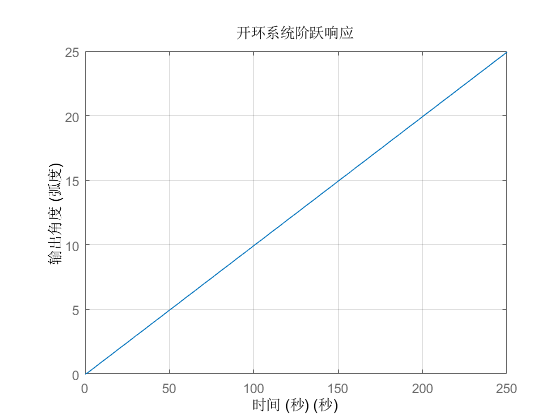
\includegraphics[width=0.8\textwidth]{fig_open_loop_step.png}
    \caption{开环系统单位阶跃响应。}
    \label{fig:open_loop}
\end{figure}

\subsection{理想全状态反馈控制器性能对比}
在假设所有状态均可直接测量的情况下,对极点配置控制器和LQR控制器的性能进行了仿真对比,如图~\ref{fig:controllers_comparison}所示,量化性能指标如表~\ref{tab:performance}所示。

\begin{figure}[htbp]
    \centering
    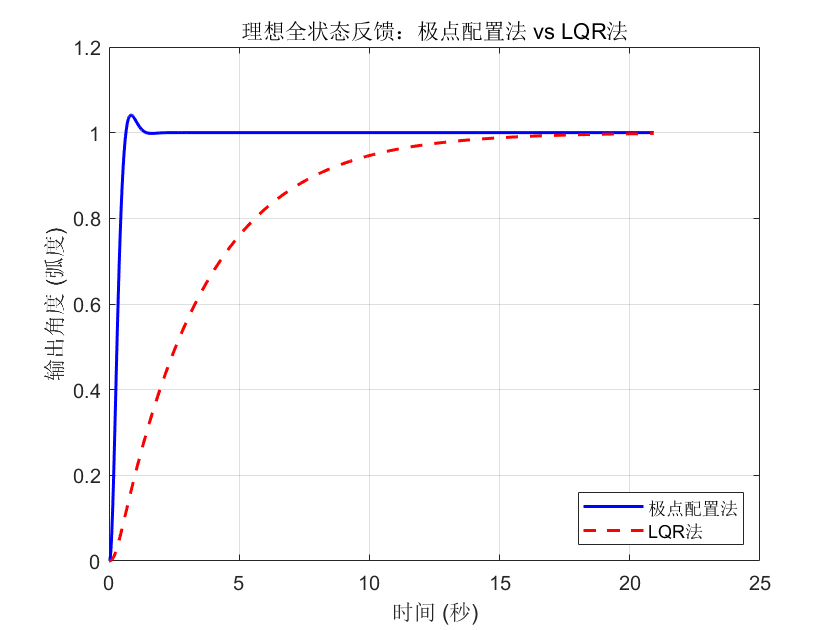
\includegraphics[width=0.9\textwidth]{fig_controllers_comparison.png}
    \caption{理想全状态反馈下,极点配置法与LQR法的阶跃响应对比。}
    \label{fig:controllers_comparison}
\end{figure}

\begin{table}[htbp]
    \centering
    \caption{两种理想控制器的量化性能指标对比。}
    \label{tab:performance}
    \begin{tabular}{lcc}
        \toprule
        \textbf{性能指标} & \textbf{极点配置法} & \textbf{LQR法} \\
        \midrule
        调节时间 (s) & 1.1050 & 13.2708 \\
        超调量 (\%) & 4.1037 & 0.0000 \\
        上升时间 (s) & 0.3968 & 7.3196 \\
        峰值 & 1.0410 & 0.9993 \\
        \bottomrule
    \end{tabular}
\end{table}

结果表明,极点配置控制器展现出极快的响应速度和较小的超调,其性能指标与设计目标高度吻合,体现了该方法“目标驱动”的特性。相比之下,LQR控制器的响应曲线更为平缓,完全没有超调,但调节时间显著增长,完美诠释了LQR在系统性能与控制成本之间进行“优化平衡”的设计哲学。

\subsection{基于状态观测器的控制系统性能分析}
为模拟实际情况,以极点配置控制器为例,构建了基于状态观测器的闭环系统,并将其性能与理想全状态反馈系统进行对比,如图~\ref{fig:observer_output}所示。

\begin{figure}[htbp]
    \centering
    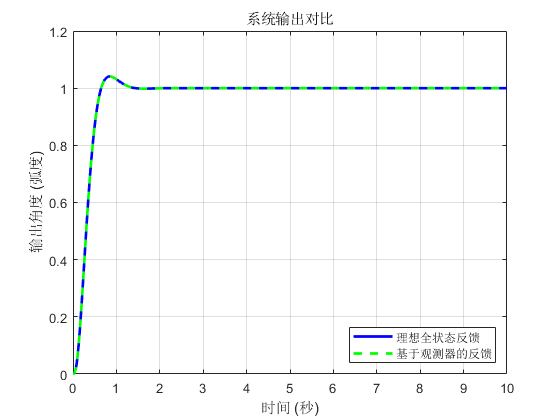
\includegraphics[width=0.9\textwidth]{fig_observer_output_comparison.png}
    \caption{理想全状态反馈与基于观测器的反馈的系统输出对比。}
    \label{fig:observer_output}
\end{figure}

从图~\ref{fig:observer_output}可以看到,基于观测器的反馈控制系统(绿色虚线)的输出响应曲线与理想全状态反馈系统(蓝色实线)的曲线几乎完全重合。这有力地验证了分离原理的正确性:只要观测器设计得当,使用估计状态进行反馈所能达到的性能可以无限逼近理想情况。为进一步验证观测器的有效性,我们对比了角速度的真实值与估计值,如图~\ref{fig:observer_estimation}所示。

\begin{figure}[htbp]
    \centering
    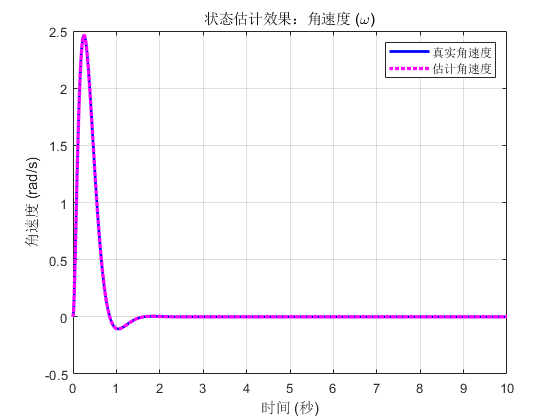
\includegraphics[width=0.9\textwidth]{fig_observer_state_estimation.png}
    \caption{角速度的真实值与估计值对比。}
    \label{fig:observer_estimation}
\end{figure}

\subsubsection{仿真结果的理想性分析}
如图~\ref{fig:observer_output}和图~\ref{fig:observer_estimation}所示,基于观测器的系统性能与理想情况几乎完全一致,估计状态也能瞬时地跟踪上真实状态。这种“完美”的结果是仿真环境高度理想化的体现,其主要原因有三:
\begin{enumerate}
    \item \textbf{模型选择:} 用于设计观测器的数学模型(矩阵$\bm{A}, \bm{B}, \bm{C}$)与用于模拟“真实”被控对象的模型完全相同。在实际工程中,模型总是存在不确定性,这种模型失配是产生估计误差的主要来源。
    \item \textbf{无噪声干扰:} 仿真环境中不存在测量噪声(如传感器读数抖动)和过程噪声(如未建模的负载扰动)。这些随机噪声在现实中会持续干扰观测器的估计精度。
    \item \textbf{极快的纠错动态:} 我们遵循设计准则,将观测器的极点配置在远快于控制器极点的位置。这使得初始的估计误差能够以极快的指数速度衰减,在宏观时间尺度上几乎不可见。
\end{enumerate}

\section{结论 (Conclusion)}
本报告成功地应用现代控制理论,为直流电机位置伺服系统设计并仿真验证了多种控制策略。研究表明:(1) 极点配置法能精确地实现预设的动态性能指标,但可能伴随较高的控制成本;(2) LQR法则能在系统性能与能量消耗之间提供一种灵活的优化平衡;(3) 状态观测器能够在仅有部分状态可测的情况下,有效估计系统全部状态,并结合状态反馈实现与理想情况几乎无异的控制效果,从而验证了分离原理的有效性。

本次基于理想化模型的仿真,为深入理解状态空间控制方法提供了坚实的基础。未来的研究可进一步考虑模型不确定性、外部扰动及测量噪声等实际因素,并引入如卡尔曼滤波器等更鲁棒的估计方法。

\section{参考文献 (References)}
\begin{thebibliography}{9}
    \bibitem{ref1} 王俊杰, 陈之浩, 方保龙, 等. 基于LQR控制算法的动量轮倒立摆设计[J]. 数字技术与应用, 2024, 42(09): 213-216.
    \bibitem{ref2} 石惠文. 基于LQR的动量轮单摆起摆及平衡控制仿真研究[J]. 科技创新与应用, 2023, 13(33): 65-68. DOI:10.19981/j.CN23-1581/G3.2023.33.016.
    \bibitem{ref3} 刘豹, 唐万生. 现代控制理论[M]. 第3版. 北京: 机械工业出版社, 2012.
\end{thebibliography}

\appendix
\section{附录 (Appendix)}
\noindent
本项目完整的MATLAB仿真代码已上传至GitHub仓库,可通过以下链接访问:
\url{https://github.com/Gan0819Han/Modern_Control_with_LQR}

\end{document}
